\documentclass[aspectratio=169,11pt]{beamer}

% Shared style, ported from the UF Animal Sciences 2026 talk (ibfe-tutorials.sty at the repo root).
\makeatletter\def\input@path{{./}{../}}\makeatother
\usepackage{ibfe-tutorials}

\usepackage[utf8]{inputenc}
\usepackage{amsmath,amssymb,bm}
\usepackage{mathtools}
\usepackage{tikz}
\usetikzlibrary{arrows.meta,positioning}

% ---------- Notation ----------
\newcommand{\x}{\bm{x}}
\newcommand{\uu}{\bm{u}}
\newcommand{\pp}{p}
\newcommand{\Rey}{\mathrm{Re}}
\newcommand{\avg}[1]{\overline{#1}}
\renewcommand{\up}{\uu'} % the style file's \up is an arrow pictogram; this deck's \up is the fluctuation
\newcommand{\ubar}{\avg{\uu}}
\newcommand{\grad}{\nabla}
\newcommand{\Div}{\nabla\cdot}
\newcommand{\Lap}{\Delta}

\title[RANS II: Momentum]{RANS Part 2: Reynolds-Averaged Momentum Equation (x-component)}
\author[Miller]{Laura A. Miller}
\institute[UArizona]{Department of Mathematics, University of Arizona}
\date{IBFE Tutorials \textbullet\ Module 5\\[3pt]
  Adapted from a \href{https://www.youtube.com/watch?v=mDt-HJEXK6g}{lecture by Steven L. Brunton}.}

\begin{document}

% ------------------------------------------------------------
\begin{frame}[plain]
\maketutorialtitle
\end{frame}

% ------------------------------------------------------------
\begin{frame}{Where we are (from Part 1)}
We start from incompressible Navier--Stokes (nondimensional):
\begin{align*}
\frac{\partial \uu}{\partial t}  + (\uu\cdot\grad)\uu &= -\grad \pp + \frac{1}{\Rey}\Lap\uu,\\
\Div\uu &= 0.
\end{align*}

Reynolds decomposition (time average):
\[
\uu(\x,t)=\ubar(\x)+\up(\x,t),\qquad \avg{\up}=0.
\]

\textbf{Result from Part 1:}
\[
\Div\ubar=0,\qquad \Div\up=0.
\]
\end{frame}

\begin{frame}{Other identities from part 1}
Recall we are taking averages in time. We know \\
\begin{align*}
\avg{u+v}=\avg{u}+\avg{v},\\
\avg{\avg{u}}=\avg{u},\\
\avg{\avg{u}\cdot v}=\avg{u}\cdot \avg{v},\\
\avg{\frac{\partial u}{\partial x}}=\frac{\partial \avg{u}}{\partial x}
\end{align*}

In general, 
\begin{align*}
\avg{u\cdot v}\neq \avg{u}\cdot \avg{v},\\
\avg{u'^2}\neq 0.
\end{align*}
\end{frame}
% ------------------------------------------------------------
\begin{frame}{Motivation: why average the momentum equation?}
Engineers often want \textbf{mean} quantities:
\begin{itemize}
  \item mean drag / mean lift,
  \item mean separation behavior,
  \item bulk transport trends,
\end{itemize}
without resolving every turbulent eddy in space-time.

\begin{block}{Plan today}
Plug $\uu=\ubar+\up$ (and $\pp=\avg{\pp}+\pp'$) into momentum,
then time-average to get an equation for $\ubar$.
\end{block}
\end{frame}

% ------------------------------------------------------------
\begin{frame}{What the averaging operation changes}
\centering
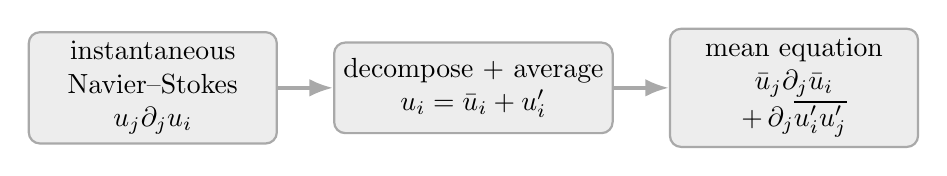
\begin{tikzpicture}[
  node distance=7mm,
  box/.style={rounded corners,draw=DarkGray,thick,fill=LightGray!40,
              minimum width=3.15cm,minimum height=1.15cm,align=center},
  arrow/.style={-{Latex[length=3mm]},very thick,DarkGray}]
  \node[box] (ns) {instantaneous\\Navier--Stokes\\$u_j\partial_j u_i$};
  \node[box,right=of ns] (avg) {decompose + average\\$u_i=\bar u_i+u'_i$};
  \node[box,right=of avg] (rans) {mean equation\\$\bar u_j\partial_j\bar u_i$\\$+\,\partial_j\overline{u'_i u'_j}$};
  \draw[arrow] (ns) -- (avg);
  \draw[arrow] (avg) -- (rans);
\end{tikzpicture}

\vspace{0.4em}
{\scriptsize\color{DarkGray} Schematic: instructor's course notes. Index notation: $u_i$ ($i=1,2,3$) are the components $(u,v,w)$, $\partial_j=\partial/\partial x_j$, and a repeated index is summed.\par}

\vspace{0.7em}
\begin{block}{The nonlinear term does not simply average away}
The correlation $R_{ij}=\overline{u'_i u'_j}$ is new information. An equation for the mean velocity alone does not determine it: this is the RANS closure problem.
\end{block}
\end{frame}

% ------------------------------------------------------------
\begin{frame}{We will derive only the x-momentum equation}
Write $\uu=(u,v,w)^T$. The x-component of momentum is:
\[
\frac{\partial u}{\partial t} + u\,\frac{\partial u}{\partial x} + v\,\frac{\partial u}{\partial y} + w\,\frac{\partial u}{\partial z}
= -\frac{\partial p}{\partial x} + \frac{1}{\Rey}\Lap u.
\]

We substitute:
\[
u=\avg{u}+u',\quad v=\avg{v}+v',\quad w=\avg{w}+w',\quad p=\avg{p}+p'.
\]
\end{frame}

% ------------------------------------------------------------
\begin{frame}{Averaging identities we will use repeatedly}
Time average operator $\avg{\cdot}$ is linear and (under mild regularity)
commutes with spatial derivatives:
\[
\avg{a+b}=\avg{a}+\avg{b},\qquad
\avg{\frac{\partial}{\partial x} a}=\frac{\partial}{\partial x} \avg{a}.
\]

Key facts:
\[
\avg{u'}=0,\qquad \avg{p'}=0,\qquad \avg{\Lap u'}=\Lap\avg{u'}=0.
\]

\begin{block}{Critical warning (the source of Reynolds stresses)}
In general,
\[
\avg{ab}\neq \avg{a}\,\avg{b}.
\]
So averages of \emph{products of fluctuations} need not vanish.
\end{block}
\end{frame}

% ------------------------------------------------------------
\begin{frame}{Step 1: substitute decomposition into x-momentum}
Start with
\[
\frac{\partial u}{\partial t} + u\,\frac{\partial u}{\partial x} + v\,\frac{\partial u}{\partial y} + w\,\frac{\partial u}{\partial z}
= -\frac{\partial p}{\partial x} + \frac{1}{\Rey}\Lap u.
\]

Substitute $u=\avg{u}+u'$, $v=\avg{v}+v'$, $w=\avg{w}+w'$, $p=\avg{p}+p'$.
Then
\begin{align*}
\frac{\partial} {\partial t}(\avg{u}+u')
&+ (\avg{u}+u')\frac{\partial}{\partial x}(\avg{u}+u')
+ (\avg{v}+v')\frac{\partial}{\partial y}(\avg{u}+u')\\
&+ (\avg{w}+w')\frac{\partial}{\partial z}(\avg{u}+u')
= -\frac{\partial}{\partial x}(\avg{p}+p') + \frac{1}{\Rey}\Lap(\avg{u}+u').
\end{align*}
\end{frame}

% ------------------------------------------------------------
\begin{frame}{Step 1a: expand the convection term (x-part shown)}
The first convection piece expands like multiplying polynomials:
\[
(\avg{u}+u')\frac{\partial}{\partial x}(\avg{u}+u')
=
\avg{u}\,\frac{\partial \avg{u}}{\partial x}
+\avg{u}\,\frac{\partial u'}{\partial x}
+u'\,\frac{\partial \avg{u}}{\partial x}
+u'\,\frac{\partial u'}{\partial x}.
\]

Similarly,
\[
(\avg{v}+v')\frac{\partial}{\partial y}(\avg{u}+u')
=
\avg{v}\,\frac{\partial \avg{u}}{\partial y}
+\avg{v}\,\frac{\partial u'}{\partial y}
+v'\,\frac{\partial \avg{u}}{\partial y}
+v'\,\frac{\partial u'}{\partial y},
\]
and likewise for the $w$-term.
\end{frame}

% ------------------------------------------------------------
\begin{frame}{Step 2: time-average the entire equation}
Time-average term-by-term.

\textbf{Time derivative:}
\[
\avg{\frac{\partial}{\partial t}(\avg{u}+u')}
=
\frac{\partial}{\partial t} \avg{u} + \frac{\partial}{\partial t}\avg{u'}
=
\frac{\partial}{\partial t} \avg{u}.
\]
For a statistically stationary mean, $\frac{\partial}{\partial t}\avg{u}=0$. Otherwise this mean-acceleration term must remain.

\textbf{Pressure and viscosity:}
\[
\avg{-\frac{\partial}{\partial x}(\avg{p}+p')}=-\frac{\partial}{\partial x}\avg{p},\qquad
\avg{\Lap(\avg{u}+u')}=\Lap\avg{u}.
\]

\textbf{Mixed mean--fluctuation products die:} e.g.
\[
\avg{\avg{u}\,\frac{\partial u'}{\partial x}}=\avg{u}\,\avg{\frac{\partial u'}{\partial x}}=0,\quad
\avg{u'\,\frac{\partial \avg{u}}{\partial x}}=\avg{u'}\,\frac{\partial \avg{u}}{\partial x}=0.
\]
What survives are \emph{mean--mean} terms and \emph{fluctuation--fluctuation} terms.
\end{frame}

% ------------------------------------------------------------
\begin{frame}{Step 2 result: averaged x-momentum (stationary mean)}
Here $\partial_x = \partial/\partial x$ etc.; subscripts are reserved for components.

After averaging, the surviving terms are:
\begin{align*}
\avg{u}\,\partial_x\avg{u}
+\avg{v}\,\partial_y\avg{u}
+\avg{w}\,\partial_z\avg{u}
&\;+\;\avg{u'\,\partial_x u'}
+\avg{v'\,\partial_y u'}
+\avg{w'\,\partial_z u'} \\
&= -\partial_x\avg{p} + \frac{1}{\Rey}\Lap \avg{u}.
\end{align*}

\begin{block}{Interpretation}
Everything is now in terms of mean fields \emph{except} the three correlation terms
$\avg{u'\,\partial_x u'}$, $\avg{v'\,\partial_y u'}$, $\avg{w'\,\partial_z u'}$.
These encode how fluctuations force the mean.
\end{block}
\end{frame}

% ------------------------------------------------------------
\begin{frame}{The problematic survivors: why they don't vanish}
Even though $\avg{u'}=0$, products of fluctuations need not average to zero:
\[
\avg{(u')^2}\neq 0,\qquad \avg{u'v'}\neq 0,\qquad \avg{u'w'}\neq 0.
\]

These are (components of) the \textbf{Reynolds stresses}.
They will become \textbf{spatial derivatives of} $\avg{(u')^2}$, $\avg{u'v'}$, $\avg{u'w'}$.

This is where closure enters: we need a model for these correlations.
\end{frame}

% ------------------------------------------------------------
\begin{frame}{Step 3: the streamwise product-rule identity}
Use the product rule:
\[
\partial_x\big((u')^2\big)=2u'\,\partial_x u'
\quad\Rightarrow\quad
u'\,\partial_x u'=\frac12\,\partial_x\big((u')^2\big).
\]

Therefore,
\[
\avg{u'\,\partial_x u'}
=
\frac12\,\frac{\partial}{\partial x}\avg{(u')^2}.
\]

This half-factor is correct for this term in isolation. In the sum of all three convective terms, continuity supplies the complementary half, as the next two slides show explicitly.
\end{frame}

% ------------------------------------------------------------
\begin{frame}{Step 3: product-rule setup for the cross terms}
Apply the product rule to $u'v'$ and $u'w'$:
\[
\frac{\partial}{\partial y}(u'v') = v'\,\partial_y u' + u'\,\partial_y v',
\qquad
\frac{\partial}{\partial z}(u'w') = w'\,\partial_z u' + u'\,\partial_z w'.
\]

Rearrange:
\[
v'\,\partial_y u' = \frac{\partial}{\partial y}(u'v') - u'\,\partial_y v',
\qquad
w'\,\partial_z u' = \frac{\partial}{\partial z}(u'w') - u'\,\partial_z w'.
\]

Now time-average:
\[
\avg{v'\,\partial_y u'} = \frac{\partial}{\partial y}\avg{u'v'} - \avg{u'\,\partial_y v'},\quad
\avg{w'\,\partial_z u'} = \frac{\partial}{\partial z}\avg{u'w'} - \avg{u'\,\partial_z w'}.
\]

These identities expose derivatives of the correlations, but they also leave two terms involving derivatives of $v'$ and $w'$. The complete vector product rule organizes all three directions at once.
\end{frame}

% ------------------------------------------------------------
\begin{frame}{Step 3: package the full convective sum}
Apply $a_j\partial_j b=\partial_j(a_jb)-b\,\partial_j a_j$ with $a_j=u'_j$ and $b=u'$:
\begin{align*}
u'\,\partial_x u'+v'\,\partial_y u'+w'\,\partial_z u'
&=\frac{\partial (u')^2}{\partial x}
 +\frac{\partial (u'v')}{\partial y}
 +\frac{\partial (u'w')}{\partial z}\\
&\quad-u'\left(\partial_x u'+\partial_y v'+\partial_z w'\right).
\end{align*}

\begin{block}{Why the half-factor disappears}
As on the streamwise slide: the product-rule correction supplies the second copy of $u'\,\partial_x u'$, so the first term is $\partial_x(u'^2)$, not $\tfrac12\partial_x(u'^2)$.
\end{block}
{\small In detail: $\partial_x(u'^2)=2u'\partial_xu'$ contains one copy too many; the extra copy is cancelled by the $-u'\partial_xu'$ inside $-u'(\Div\up)$. That whole bracket vanishes only because all three of its pieces are kept together, which is why the cross terms must be treated in the same step.\par}
\end{frame}

% ------------------------------------------------------------
\begin{frame}{The cancellation: use $\Div \up = 0$}
The correction in the packaged identity is
\[
\avg{u'\,\partial_x u'}+\avg{u'\,\partial_y v'}+\avg{u'\,\partial_z w'}.
\]

Factor out $u'$:
\[
u'\,\partial_x u' + u'\,\partial_y v' + u'\,\partial_z w'
=
u'\,(\partial_x u'+\partial_y v'+\partial_z w')
=
u'\,(\Div\up).
\]

But from Part 1, $\Div\up=0$, hence
\[
\avg{u'\,\partial_x u'}+\avg{u'\,\partial_y v'}+\avg{u'\,\partial_z w'}=0.
\]

The correction vanishes, so no factor of $\tfrac12$ is missing (see the streamwise slide).
\end{frame}

% ------------------------------------------------------------
\begin{frame}{Step 3 result: the Reynolds-stress-gradient form}
Using the identities and cancellations, the fluctuation terms become:
\[
\avg{u'\,\partial_x u'}+\avg{v'\,\partial_y u'}+\avg{w'\,\partial_z u'}
=
\frac{\partial}{\partial x}\avg{(u')^2}
+\frac{\partial}{\partial y}\avg{u'v'}
+\frac{\partial}{\partial z}\avg{u'w'}.
\]

Equivalently, in index notation,
\[
\overline{u'_j\partial_j u'_i}
=\partial_j\overline{u'_i u'_j}
-\overline{u'_i\partial_j u'_j}
=\partial_j R_{ij},
\]
because $\partial_j u'_j=0$.
\end{frame}

% ------------------------------------------------------------
\begin{frame}{Final x-component RANS equation (stationary mean)}
The Reynolds-averaged x-momentum equation can be written as:
\begin{align*}
\avg{u}\,\partial_x\avg{u}
+\avg{v}\,\partial_y\avg{u}
+\avg{w}\,\partial_z\avg{u}
&=
-\partial_x\avg{p}
+\frac{1}{\Rey}\Lap\avg{u}
-\Big(
\frac{\partial}{\partial x}\avg{(u')^2}
+\frac{\partial}{\partial y}\avg{u'v'}
+\frac{\partial}{\partial z}\avg{u'w'}
\Big).
\end{align*}

\begin{block}{Key interpretation}
The mean flow is driven by pressure + viscosity \emph{and} the divergence of Reynolds stresses.
\end{block}
\end{frame}

% ------------------------------------------------------------
\begin{frame}{The general unsteady RANS equation}
If the averaging operation produces a time-dependent mean, retain its time derivative:
\[
\frac{\partial \bar u_i}{\partial t}
+\bar u_j\frac{\partial \bar u_i}{\partial x_j}
=-\frac{\partial \bar p}{\partial x_i}
+\frac{1}{\Rey}\Delta\bar u_i
-\frac{\partial R_{ij}}{\partial x_j},
\qquad
\frac{\partial \bar u_j}{\partial x_j}=0.
\]

\begin{block}{Stationary specialization}
The preceding derivation set $\partial_t\bar u_i=0$ only after explicitly assuming statistically stationary mean fields. Reynolds averaging itself does not require this term to vanish.
\end{block}
\end{frame}

% ------------------------------------------------------------
\begin{frame}{Vector/tensor form (what this looks like in compact notation)}
Define the velocity-correlation tensor:
\[
\bm{R} := \avg{\up\,\up^{T}}
=
\begin{bmatrix}
\avg{u'u'} & \avg{u'v'} & \avg{u'w'}\\
\avg{v'u'} & \avg{v'v'} & \avg{v'w'}\\
\avg{w'u'} & \avg{w'v'} & \avg{w'w'}
\end{bmatrix}.
\]

Then the stationary mean momentum equation is commonly written:
\[
(\ubar\cdot\grad)\ubar
=
-\grad \avg{p}
+\frac{1}{\Rey}\Lap \ubar
-\Div \bm{R}.
\]

Along with mean incompressibility: \;\; $\Div\ubar=0$.
\end{frame}

% ------------------------------------------------------------
\begin{frame}{Correlation tensor versus turbulent stress}
The term $-\Div\bm{R}$ acts like an additional forcing in the nondimensional mean equation, with the same differential form as a stress divergence.

\begin{itemize}
  \item $R_{ij}=\avg{u'_i u'_j}$ is a velocity-correlation tensor.
  \item In dimensional form, the corresponding turbulent (Reynolds) stress is commonly defined as $\tau^{R}_{ij}=-\rho R_{ij}$; some texts instead call $\rho R_{ij}$ the Reynolds-stress tensor and keep the minus sign in the equation.
  \item These are not determined by the mean equation alone.
\end{itemize}

\begin{block}{Closure problem (core of RANS modeling)}
The averaged equations introduce new unknowns ($\bm{R}$) that require modeling:
\[
\bm{R} \approx \mathcal{M}(\ubar, \grad \ubar, \ldots).
\]
\end{block}
\end{frame}

% ------------------------------------------------------------
\begin{frame}{What comes next (closure + ML)}
Next topics in a RANS sequence:
\begin{itemize}
  \item classic closures (e.g., eddy viscosity / Boussinesq hypothesis),
  \item $k$--$\varepsilon$, $k$--$\omega$, Spalart--Allmaras, etc.
  \item data-driven closure ideas (ML approximations of $\bm{R}$ or corrections).
\end{itemize}

\begin{block}{Takeaway}
RANS reduces space-time complexity, but pays a price: \textbf{closure modeling}.
\end{block}
\end{frame}

% ------------------------------------------------------------
\begin{frame}{Worked check: fully developed channel flow}
Take a statistically stationary, fully developed channel, $\avg{u}=\avg{u}(y)$, $\avg{v}=\avg{w}=0$, with statistics independent of $x$ and $z$.
\begin{itemize}
  \item The left side $\avg{u}\,\partial_x\avg{u}+\avg{v}\,\partial_y\avg{u}+\avg{w}\,\partial_z\avg{u}$ vanishes term by term.
  \item Of the Reynolds-stress terms only $\partial_y\avg{u'v'}$ survives, so the final x-equation becomes
  \[
    0=-\partial_x\avg{p}+\frac1{\Rey}\frac{\mathrm d^2\avg{u}}{\mathrm dy^2}-\frac{\mathrm d}{\mathrm dy}\avg{u'v'}.
  \]
  \item The y-equation gives $\avg{p}+\avg{v'^2}$ independent of $y$, so $\partial_x\avg{p}$ is a constant and the \emph{total} shear stress
  $\frac1{\Rey}\frac{\mathrm d\avg{u}}{\mathrm dy}-\avg{u'v'}$ is linear in $y$.
\end{itemize}
\begin{block}{Interpretation}
Near the wall the viscous part carries the stress; away from it the Reynolds shear stress $-\avg{u'v'}$ does. This is the starting point of the wall-scaling and log-law slides in deck 5-3 (see also Pope 2000, \S7.1).
\end{block}
\end{frame}

% ------------------------------------------------------------
\begin{frame}{Summary}
\begin{itemize}
  \item Start with x-momentum component of incompressible Navier--Stokes.
  \item Substitute $\uu=\ubar+\up$ and time-average.
  \item Mixed mean--fluctuation terms vanish; products of fluctuations remain.
  \item Use product-rule identities + $\Div\up=0$ to package surviving terms as
  \[
  -\left(\frac{\partial}{\partial x}\avg{(u')^2}+\frac{\partial}{\partial y}\avg{u'v'}+\frac{\partial}{\partial z}\avg{u'w'}\right)
  = -(\Div \bm{R})_x.
  \]
  \item The resulting mean equation requires a closure model for $\bm{R}$.
\end{itemize}
\end{frame}

% ------------------------------------------------------------
\begin{frame}{References and sign convention}
\small
\begin{itemize}
  \item O. Reynolds, ``On the dynamical theory of incompressible viscous fluids and the determination of the criterion,'' \emph{Philosophical Transactions of the Royal Society A}, 186 (1895).
  Pages 123--164; \href{https://doi.org/10.1098/rsta.1895.0004}{doi:10.1098/rsta.1895.0004}.
  \item S. B. Pope, \emph{Turbulent Flows}, Cambridge University Press (2000), Chapters 3--4.
  \item S. L. Brunton, lecture on Reynolds-averaged Navier--Stokes equations.
  \href{https://www.youtube.com/watch?v=mDt-HJEXK6g}{YouTube} (the video linked from Part~1; the derivation sequence of this deck is adapted from Brunton's RANS lecture material).
  \item D. C. Wilcox, \emph{Turbulence Modeling for CFD}, 3rd ed., DCW Industries (2006), Ch.~2 (Reynolds averaging and the Reynolds-stress tensor; alternative sign conventions).
\end{itemize}

\begin{block}{Convention used here}
$R_{ij}=\overline{u'_i u'_j}$ is the velocity-correlation tensor, so the nondimensional RANS equation contains $-\partial_jR_{ij}$. In dimensional stress notation, $\tau^R_{ij}=-\rho R_{ij}$ and the same contribution is $\rho^{-1}\partial_j\tau^R_{ij}$.
\end{block}
\end{frame}

\end{document}
